\documentclass[12pt,a4paper]{article}
\usepackage[]{graphicx}
\usepackage[]{color}
\usepackage{chngcntr}
\usepackage{pdfpages}
\usepackage{pdflscape}
\usepackage{subfig}
\usepackage[backend=biber]{biblatex}
\addbibresource{biblio.bib}
\usepackage[
colorlinks,
citecolor=blue,
urlcolor=cyan,
bookmarks=true,
hypertexnames=true
]{hyperref}
\usepackage{alltt}
\usepackage{arxiv}
\usepackage[utf8]{inputenc} % allow utf-8 input
\usepackage[T1]{fontenc}    % use 8-bit T1 fonts
\usepackage{url}            % simple URL typesetting
\usepackage{booktabs}       % professional-quality tables
\usepackage{amsfonts}       % blackboard math symbols
\usepackage{nicefrac}       % compact symbols for 1/2, etc.
\usepackage{microtype}      % microtypography
\usepackage{setspace}

% Stuff for the table
\usepackage{array, booktabs, caption, pdflscape, makecell, siunitx, multirow, caption}
\renewcommand\theadfont{\bfseries}
\setcounter{table}{0}
\renewcommand{\thetable}{S\arabic{table}}
\setlength\extrarowheight{7pt}

\renewcommand{\thesection}{S\arabic{section}}
%\renewcommand{\thesubsection}{\thesubsection.S\arabic{subsection}}

% maxwidth is the original width if it is less than linewidth
% otherwise use linewidth (to make sure the graphics do not exceed the margin)
\makeatletter
\def\maxwidth{ %
  \ifdim\Gin@nat@width>\linewidth
    \linewidth
  \else
    \Gin@nat@width
  \fi
}
\makeatother

\definecolor{fgcolor}{rgb}{0.345, 0.345, 0.345}
\newcommand{\hlnum}[1]{\textcolor[rgb]{0.686,0.059,0.569}{#1}}%
\newcommand{\hlstr}[1]{\textcolor[rgb]{0.192,0.494,0.8}{#1}}%
\newcommand{\hlcom}[1]{\textcolor[rgb]{0.678,0.584,0.686}{\textit{#1}}}%
\newcommand{\hlopt}[1]{\textcolor[rgb]{0,0,0}{#1}}%
\newcommand{\hlstd}[1]{\textcolor[rgb]{0.345,0.345,0.345}{#1}}%
\newcommand{\hlkwa}[1]{\textcolor[rgb]{0.161,0.373,0.58}{\textbf{#1}}}%
\newcommand{\hlkwb}[1]{\textcolor[rgb]{0.69,0.353,0.396}{#1}}%
\newcommand{\hlkwc}[1]{\textcolor[rgb]{0.333,0.667,0.333}{#1}}%
\newcommand{\hlkwd}[1]{\textcolor[rgb]{0.737,0.353,0.396}{\textbf{#1}}}%
\let\hlipl\hlkwb

\usepackage{framed}
\makeatletter
\newenvironment{kframe}{%
 \def\at@end@of@kframe{}%
 \ifinner\ifhmode%
  \def\at@end@of@kframe{\end{minipage}}%
  \begin{minipage}{\columnwidth}%
 \fi\fi%
 \def\FrameCommand##1{\hskip\@totalleftmargin \hskip-\fboxsep
 \colorbox{shadecolor}{##1}\hskip-\fboxsep
     % There is no \\@totalrightmargin, so:
     \hskip-\linewidth \hskip-\@totalleftmargin \hskip\columnwidth}%
 \MakeFramed {\advance\hsize-\width
   \@totalleftmargin\z@ \linewidth\hsize
   \@setminipage}}%
 {\par\unskip\endMakeFramed%
 \at@end@of@kframe}
\makeatother

\definecolor{shadecolor}{rgb}{.97, .97, .97}
\definecolor{messagecolor}{rgb}{0, 0, 0}
\definecolor{warningcolor}{rgb}{1, 0, 1}
\definecolor{errorcolor}{rgb}{1, 0, 0}
\newenvironment{knitrout}{}{} % an empty environment to be redefined in TeX

\newcommand{\I}{\mathbb{I}}

\title{Long-term demographic dynamics of a keystone scavenger disrupted by
	human-induced shifts in food availability}


\author{
	Pablo Almaraz
	\\
	Department of Ecology and Coastal Management, \\
	ICMAN-CSIC, \\
	Campus Río San Pedro, 11510, Puerto Real, Spain.\\  \texttt{\href{mailto:pablo.almaraz@csic.es}{\nolinkurl{pablo.almaraz@csic.es}}} \\
	\And
	Félix Martínez
	\\
	Sociedad para la Conservación de los Vertebrados, \\
	Avda. de los Pinos 17, 58B, ES-28914 Leganés, Madrid, Spain. \\
	\texttt{} \\
	\And
	Zebensui Morales-Reyes
	\\
	Departamento de Biología Aplicada, \\
	Universidad Miguel Hernández \\
	Avda. de la Universidad, s/n, 03202 Elche, Alicante, Spain. \\
	\texttt{} \\
	\And
	José A. Sánchez-Zapata
	\\
	Departamento de Biología Aplicada \\
	Universidad Miguel Hernández \\
	Avda. de la Universidad, s/n, 03202 Elche, Alicante, Spain. \\
	\texttt{} \\
	\And
	Guillermo Blanco
	\\
	Department of Evolutionary Ecology \\
	MNCN-CSIC \\
	José Gutiérrez Abascal 2, 28006 Madrid, Spain. \\
	\texttt{} \\
}

\IfFileExists{upquote.sty}{\usepackage{upquote}}{}
\begin{document}

\large{\textbf{Supporting Information}. Almaraz, P., Martínez, F., Morales-Reyes, Z., Sánchez-Zapata, J. A., Blanco, G. 2021. Long-term demographic dynamics of a keystone scavenger disrupted by human-induced shifts in food availability. Ecological Applications.}

\vspace{0.7in}

%\maketitle

\tableofcontents
%\counterwithin{figure}{section}

%\newpage

\vspace{0.7in}

\def\tightlist{}

\section{The inverse Bayesian demographic model}

Here we outline in more detail the mathematical and statistical construction of the inverse state-space, stage-structured density-dependent demographic model (hereafter S4D3M). A life-cycle graph of the model is represented in Figure \ref{fig:FigLifeCycle}.\\

\renewcommand{\thefigure}{S1}
\begin{figure}[htbp]
	\begin{center}
		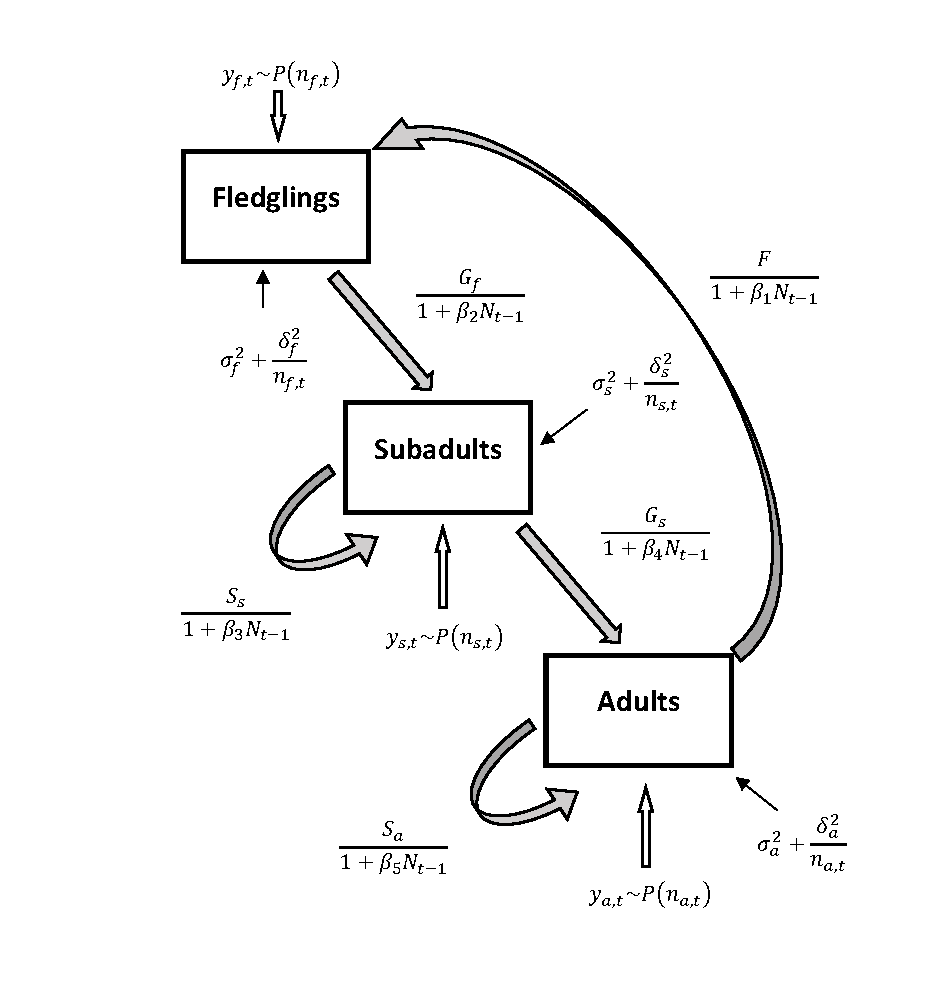
\includegraphics[width=10cm]{figs/FigS1.pdf}
	\end{center}
	\caption{Life-cycle graph for the Eurasian griffon vulture with three sequential life stages (fledglings, sub-adults and adults) linked by thick gray arrows, and five density-dependent vital rates. The true (latent) abundances of fledglings ($n_{f,t}$), sub-adults ($n_{s,t}$) and adults ($n_{a,t}$) are linked to the observed abundances (the data; $y_{f,t}$, $y_{s,t}$, $y_{a,t}$, respectively) through an observation model (open arrows). This accounts for errors in the assignment of a demographic stage to the monitored individuals. An average fledgling enters the sub-adult stage with a probability ($G_{f}$; fledgling recruitment). Once in that stage, it may either survive as a sub-adult with a probability ($S_{s}$; sub-adult survival), or enter the adult population with a transition probability ($G_{s}$; sub-adult recruitment). Finally, an adult may survive with a probability ($S_{a}$; adult survival) and breed with an average fecundity ($F$; fecundity), which closes the graph. A stochastic term including both environmental ($\sigma_{i}^2$) and demographic stochasticity ($\delta_{i}^2$) impacts each life-stage. $ N_{t-1} $ is the total population size at time $t-1$.}
\label{fig:FigLifeCycle}
\end{figure}

\subsection{The full state-space specification}

The state-space model used in the present paper is composed of a set of state equations, representing the temporal dynamics of each stage according to a set of vital rates and both demographic and environmental stochastic noise. In full matrix form this state equations can be written as:

\begin{align}\label{FullModel}
	\left(\begin{array}{c}{n_{f, t}} \\ {n_{s, t}} \\ {n_{a, t}}\end{array}\right)=
	\left(\begin{array}{ccc}{0} & {0} & {\frac{F}{1+\beta_{1} N_{t-1}}} \\
		{\frac{G_{f}}{1+\beta_{2} N_{t-1}}} & {\frac{S_{s}}{1+\beta_{3} N_{t-1}}} & {0} \\
		{0} & {\frac{G_{s}}{1+\beta_{4} N_{t-1}}} & {\frac{S_{a}}{1+\beta_{5} N_{t-1}}}\end{array}\right)
	\times\left(\begin{array}{c}{n_{f, t-1}} \\ {n_{s, t-1}} \\ {n_{a, t-1}}\end{array}\right)+ \notag \\
	MVN\left(0,\left(\begin{array}{ccc}{\sigma_{f}^{2}} & {\zeta_{f, s}} & {\zeta_{f, a}} \\
		{\zeta_{s, f}^{2}} & {\sigma_{s}^{2}} & {\zeta_{s, a}^{2}} \\
		{\zeta_{a, f}} & {\zeta_{a, s}} & {\sigma_{a}^{2}}\end{array}\right)+\left(\begin{array}{ccc}{\frac{\delta_{f}^{2}}{n_{f, t}}} & {0} & {0} \\
		{0} & {\frac{\delta_{s}^{2}}{n_{s, t}}} & {0} \\
		{0} & {0} & {\frac{\delta_{a}^{2}}{n_{a, t}}}\end{array}\right)\right)
\end{align}

The observations made on each stage at each time $t$, $y_{f,t}, y_{s,t}$ and $y_{a,t}$, are linked to the latent sates of the set of state equations in \ref{FullModel}, $n_{f,t}, n_{s,t}$ and $n_{a,t}$, through a second set of observation equations:

\begin{equation}\label{ObsEqns}
	\begin{array}
		{l}{y_{f, t} \sim \mathcal{P}(n_{f, t})} \\
		{y_{s, t} \sim \mathcal{P}(n_{s, t})} \\
		{y_{a, t} \sim \mathcal{P}(n_{a, t})}
	\end{array}
\end{equation}

Finally, the model is fully specified with a set of initial conditions for each latent sate. In this case, the initial observations for each state are used as the priors for the initial states:

\begin{equation}\label{InitStat}
	\begin{array}
		{l}{n_{f, 1} \sim \mathcal{P}(y_{f, 1})} \\
		{n_{s, 1} \sim \mathcal{P}(y_{s, 1})} \\
		{n_{a, 1} \sim \mathcal{P}(y_{a, 1})}
	\end{array}
\end{equation}

Overall, the set of equations in \ref{FullModel}-\ref{InitStat} represent a non-linear, non-Gaussian state-space model \cite{Durbin2001}. The S4D3M is non-linear due to the density-dependent specification of the vital rates, and it is non-Gaussian due to the Poisson distribution specified for the observation equations and initial states.\\

\subsection{Prior specification}

We performed a literature review for assembling a database of natural history data on vital rates estimates of wild Eurasian Griffon vultures. The data assembled from the literature is shown in Table \ref{t_sim}. We used this information to construct weakly informative priors for each vital rate. The average meta-analytic adult survival compiled from the literature, $S_{a}$, as well as the meta-analytic variance in adult survival, $\sigma^2S_{a}$ (see Table \ref{t_sim}) were used as the mean and variance for the prior distribution. To allow the Bayesian MCMC scheme to explore a wider range of the posterior distribution, a 10-fold increased prior variance was used. Thus, taking into account that survival is a probability, the distribution takes the form of a normal distribution truncated at (0, 1), $S_{a} \sim \textnormal{N}(\bar S_{a}, 10 \times \sigma^2S_{a})T(0,1)$, where $T(a, b)$ denotes truncation at $a$ and $b$. This strategy of prior specification was used for the rest of vital rates: the prior for fledgling recruitment ($G_{f}$) was specified as $G_{f} \sim \textnormal{N}(\bar G_{f}, 10 \times \sigma^2G_{f})T(0,1)$. The brood size of the Eurasian griffon vulture is of a single fledgling, so a normal distribution truncated at 0 and 1 was implemented for fecundity. We took advantage of the fecundity data compiled in our study area during the 42-year period to construct the prior for fecundity; since the maximum number of fledglings per breeding pair is 1, the prior for fecundity was specified as $F \sim \textnormal{N}(\bar{F}, \sigma^2{F})T(0,1)$. Finally, sub-adult recruitment ($G_{s}$) and survival ($S_{s}$), represent probabilities of transition from the same stage; that is, assuming no emigration, a sub-adult can either remain as a sub-adult, or survive to the adult stage. Therefore, both rates are not independent since their sum must be = 1, and they are constrained to be positive. A Dirichlet (1,1) distribution, which is the continuous multivariate generalization of the beta distribution, is traditionally used as priors for these rates (e.g., \cite{Gross2002}). In our case, we take advantage of the natural history data on sub-adult survival available in the literature (Table \ref{t_sim}) and implement a truncated normal prior distribution for sub-adult survival, $S_{s} \sim \textnormal{N}(\bar S_{s}, 10 \times \sigma^2S_{s})T(0,1)$. We thus model sub-adult recruitment as $G_{s} = 1 - S_{s}$.\\

The covariance matrix for environmental noise in $\Sigma_{t}$ (C) was modeled with a scaled inverse Wishart distribution (\cite{Huang2013}), $C^{-1} \sim \textnormal{SWishart}(\zeta, S)$. While the  inverse Wishart distribution is the conjugate prior for the covariance matrix of a multivariate normal distribution (\cite{Gelman2014}), it is known to severely constrain the variance parameters. In contrast, the scaled inverse Wishart, also known as the Huang-Wand distribution (\cite{Huang2013}), allows for the separate estimation of a diagonal matrix of scale parameters ($\zeta$) and an unscaled covariance matrix ($S$) following the Wishart distribution. Interestingly, with this distribution the standard deviation and correlation parameters are marginally non-informative, in contrast to the inverse Wishart (see \cite{Huang2013}), and still conditionally conjugate on the expanded space. The same prior scale ($\boldsymbol{\zeta} = \I$) was placed on all the elements of the variance-covariance matrix. The number of degrees of freedom was set to the number of stages, $S$ = 3, which is the value placing marginal uniform distributions on the correlation parameters of the covariance matrix ($S \sim \textnormal{U}(0,1)$). Finally, prior uniform distributions were placed on the standard deviation of demographic noise for each stage, $\delta_{i} \sim \textnormal{U}(0,10)$. \\

\section{Evaluating the evidence for density-dependence in the life-cycle}

The monitored population of Eurasian Griffon vulture showed a steady increasing trend during the 42-year period, only interrupted by the BSE outbreak and the corresponding sanitary legislation. However, given the long time period considered, it is highly likely that density-dependent processes were operating on some vital rates. The state-space model constructed (Eqns. \ref{FullModel}-\ref{InitStat}) is relatively complex in terms of number of parameters, with non-linear density-dependent terms in the demographic transitions among stages. To control for potential issues with MCMC convergence and posterior cross-correlations among parameters, we used a regularization (sparsity-inducing) scheme on the density-dependent parameters impacting on each vital rate, $\beta_{i}$. In brief, with regularization methods it is possible to set some parameters to 0 during the MCMC simulation if their effects on the posterior probability is negligible, and simultaneously let the simulation scheme to estimate freely those parameters with non-negligible effects on the posterior (see \cite{OHara2009} for an introduction to regularization methods, and \cite{Almaraz2011,Mutshinda2011} for ecological examples). \\

Here we use a Stochastic Search Variable Selection scheme (SSVS; \cite{George1993}) to automatically set close to 0 the density-dependent parameters with a negligible effect on demography during the MCMC simulation. Specifically, we used a spike-and-slab prior in the following distribution for the $\beta_{i}$'s in the demographic model:

\begin{equation}\label{dd_dist}
	\beta_{i} \sim \textnormal{N}(0, \tau_{i}^2)T(0,\infty)
\end{equation}

Note that this parameter can only take positive values, so it is truncated at 0. The hyperprior for the variance of the parameter $\beta_{i}$, $\tau_{i}^2$, is further modeled as:

\begin{equation}\label{ssvs}
	\tau_{i}^2 = (1 - p_{i}) \times \sigma_{0}^2 + p_{i} \times \sigma_{1}^2
\end{equation}

were $p_{i}$ is the probability that a given density-dependent parameter is included in the model, while the constants $\sigma_{0}^2$ and $\sigma_{1}^2$ are the variance when the parameter is either not-included or included in the model, respectively. We set these variances to $\sigma_{0}^2 = 10^{-4}$ and $\sigma_{1}^2 = 0.1$ (see below). Finally, the probabilities of inclusion of a given parameter, $p_{i}$, are given a Bernoulli distribution,

\begin{equation}\label{dist_bern}
	p_{i} \sim \textnormal{Bern}(\rho)
\end{equation}

where $\rho$ is the prior probability of inclusion of the density-dependent parameters. Recall that a Bernoulli distribution can only take two values, either 0 or 1. In previous approaches a given constant was used as the prior $\rho$ (e.g., 0.2; see \cite{Almaraz2011,Mutshinda2011}). Here, we used a weakly informative beta distribution for $\rho$ to let the model to learn from sparsity during the posterior simulation:

\begin{equation}\label{dist_beta}
	\rho \sim \textnormal{beta}(2,2)
\end{equation}

The beta distribution is a family of distributions defined on the continuous interval [0, 1]. They are parameterized by two shape parameters, and it is the conjugate prior of the Bernoulli distribution \cite{Gelman2014}. In our case, a $\textnormal{beta}(2,2)$ is weakly informative centered on 0.5; this stabilized the posterior simulation. In contrast, one can use a $\textnormal{beta}(1,1)$ as a completely uninformative distribution. Indeed, this later distribution is just a uniform probability distribution defined on the [0, 1] interval.\\

Overall, if the probability of inclusion $p_{i}$ of a given density-dependent parameter $\beta_{i}$ is 1 during the simulation, according to some prior $\rho$, this means that this parameter is active, so its variance (eqn. \ref{ssvs}) becomes $\tau_{i}^2 = p_{i} \times \sigma_{1}^2 = 0.1$, and the prior for the density-dependent parameter is converted into $\beta_{i} \sim \textnormal{N}(0, 0.1)T(0,\infty)$. This is the slab. On the other hand, if the probability of inclusion $p_{i}$ of a given density-dependent parameter $\beta_{i}$ is 0, this parameter is inactivated because, in this case, $\tau_{i}^2 = (1 - p_{i}) \times \sigma_{0}^2 = 10^{-4}$, and then the prior for the density-dependent parameter is converted into $\beta_{i} \sim \textnormal{N}(0, 10^{-4})T(0,\infty)$. This is the spike. During the posterior simulation, those density-dependent parameters $\beta_{i}$ significantly affecting the posterior distribution will more often be in an activated state. This means that the posterior probability of inclusion of a given parameter in the model is simply the proportion of times that the parameter was activated during the MCMC simulation (that is, the number of times that $p_{i} = 1$). This posterior probability can be compared to the prior probability of inclusion, $\rho$, which is common to all parameters (more specifically, to the posterior of the prior inclusion probability). This is very convenient, because a Bayes factor, $\textnormal{BF}_{i}$, \cite{Kass1995,Almaraz2011,Mutshinda2011} can then be calculated for every density-dependent parameter in the life-cycle:

\begin{equation}
	\textnormal{BF}_{i} =  \frac{p_{i}}{1-p_{i}} \times \frac{\rho}{1-\rho}
\end{equation}

According on the Kass-Raftery scale \cite{Kass1995}, it is possible to evaluate the evidence in favor of the inclusion of a given density-dependent parameter in the demographic model based on its Bayes factor.\\

\section{Variance component estimation}

Given the availability of a 42-year database of time-series abundance data it is straightforward to estimate the relative contribution of each vital rate and stochastic component in the stage-structured model to the observed temporal variance in population dynamics (see also \cite{Almaraz2011,Mutshinda2011}). A variance component was derived for the temporal variance in the abundance of each demographic stage \textit{i} ($var_{i}$). Denoting the temporal variance of the demographic stage \textit{i} as $\sigma^2_{n_{i}}$, and the temporal variance of the total population size as $\sigma^2_{N}$, this partitioning is:

\begin{equation}\label{VarCompSingle}
	\begin{array}{l}
		{var_{f} = \frac{F^{2}\sigma^2_{n_{a}}}{\left(1 + \beta_{1}\sigma^2_{N}\right)^2} + \sigma_{f}^{2}+\frac{\delta_{f}^{2}}{\sigma^2_{n_{f}}}} \\
		
		{var_{s} = \frac{G_{f}^{2}\sigma^2_{n_{f}}}{\left(1 + \beta_{2}\sigma^2_{N}\right)^2} + \frac{S_{s}^{2}\sigma^2_{n_{s}}}{\left(1 + \beta_{3}\sigma^2_{N}\right)^2} + \sigma_{s}^{2}+\frac{\delta_{s}^{2}}{\sigma^2_{n_{s}}}} \\
		
		{var_{a} = \frac{G_{s}^{2}\sigma^2_{n_{s}}}{\left(1 + \beta_{4}\sigma^2_{N}\right)^2} + \frac{S_{a}^{2}\sigma^2_{n_{a}}}{\left(1 + \beta_{5}\sigma^2_{N}\right)^2} + \sigma_{a}^{2} + \frac{\delta_{a}^{2}}{\sigma^2_{n_{a}}}}
	\end{array}
\end{equation}

for the fledgling (\textit{f}), sub-adult (\textit{s}) and adult stages (\textit{a}), respectively. The total temporal variance of the stage-structured population, $Var_{T}$ is just the sum of each of the above component. This total variance can thus be partitioned into the additive variance components of each demographic stage of the Lefkovitch matrix and both the environmental and demographic stochastic components in eqn. \ref{FullModel}:

\begin{align}\label{VarCompFull}
	Var_{T}=
	\underbrace{\frac{F^{2}\sigma^2_{n_{a}}}{\left(1 + \beta_{1}\sigma^2_{N}\right)^2}}_{\text{Fecundity}} +
	\underbrace{\frac{G_{f}^{2}\sigma^2_{n_{f}}}{\left(1 + \beta_{2}\sigma^2_{N}\right)^2}}_{\text{Fledgling recruitment}} +
	\underbrace{\frac{S_{s}^{2}\sigma^2_{n_{s}}}{\left(1 + \beta_{3}\sigma^2_{N}\right)^2}}_{\text{Sub-adult survival}} +
	\underbrace{\frac{G_{s}^{2}\sigma^2_{n_{s}}}{\left(1 + \beta_{4}\sigma^2_{N}\right)^2}}_{\text{Sub-adult recruitment}} +
	\notag\\
	\underbrace{\frac{S_{a}^{2}\sigma^2_{n_{a}}}{\left(1 + \beta_{5}\sigma^2_{N}\right)^2}}_{\text{Adult survival}} +
	\underbrace{\sum_{i=f}^{a} \sigma_{i}^{2}}_{\text{Environmental stochasticity}} +
	\underbrace{\sum_{i=f}^{a} \frac{\delta_{i}^{2}}{\sigma^2_{n_{i}}}}_{\text{Demographic stochasticity}}
\end{align}

\vspace{0.2in}

\section{Equilibrium population size and stability of the density-dependent model}

The transient rate of increase of a stage-structured population growing according to the S4D3M in eqns. \ref{FullModel}-\ref{InitStat} is defined as the rate at which the population grows when it is not at equilibrium; that is, whenever $N_{t} \neq N^* \quad \forall t$. When the population is at equilibrium, the population growth rate is, by definition, 0, since $N_{t + \Delta t} = N_{t} \quad \forall \Delta t, t$. If a population persists indefinitely in a stochastic environment, the asymptotic, long-term rate of increase ($\lambda_{s}$, see \cite{Caswell2001}) is a probability distribution with an average around 1, $\bar \lambda_{s} \approx 1$. In particular, the asymptotic long-term population growth rate in stochastic environments is the logarithm of the asymptotic rate of increase ($log \lambda_{s} \approx 0$) for persistent populations (see \cite{Caswell2010,Caswell2019}), but we focus here in the asymptotic rate of increase. Therefore, in a density-dependent regulated population growing in a stochastic environment stability is achieved whenever $\bar \lambda_{s} \approx 1$. Then, the frequency distribution of population sizes for which $\bar \lambda_{s} \approx 1$ in the long term is, indeed, the population at equilibrium, $N^*$. Note that we are always making a fundamental distinction between deterministic environments with analytic solutions (in which the asymptotic rate of increase $\lambda$ is exactly 1), and stochastic environments with inverse numeric solutions, in which $\lambda_{s}$ is a probability distribution centered around 1. \\

Analytically it is relatively straightforward to estimate the population at equilibrium, $N^*$, from the demographic model in eqns. \ref{FullModel}-\ref{InitStat}. However, we take advantage of the inverse state-space Bayesian approach and calculate $N^*$ numerically: we preliminary fitted the S4D3M to the stage-structured time series for each period, and then simulated the fitted model for an additional 200-year period into the future until the population stabilized. The equilibrium population size $N^*$ for each time period is then the posterior simulated distribution for the total population size after stabilization. These simulated posteriors are shown in Figure \ref{fig:Neqs}.\\

The posterior distributions of the asymptotic rates of increase ($\lambda_{s}$) of the stage-structured populations evaluated at the equilibrium $N^*$ are shown in the accompanying paper. Interestingly, in spite of the impact of different sources of observational and process stochasticity on the dynamics, the distributions are centered around 1, which suggests that the stage-structured Eurasian Griffon vulture population is stabilized in the long-term. \\

Finally, it is interesting to evaluate the dynamical stability (stability in the Liapunov's sense, \cite{Elaydi2005}) of the S4D3M evaluated at the equilibrium $N^*$. Under some assumptions (see \cite{Caswell2001,Elaydi2005}) it is possible to use a version of the S4D3M linearized around the equilibrium $N^*$ to inform about the local, linear stability of the dynamics at this point. This is achieved through the construction of the Jacobian matrix, which is the first term of a Taylor expansion of an analytical function around a given point. It is constructed by finding the partial derivatives of all the functions in the model to the state variables (see \cite{Caswell2001} and \cite{Otto2011} for a gentle introduction). In our case, the Jacobian matrix is derived by Taylor-expanding the Lefkovitch matrix in eqn. \ref{FullModel} around the equilibrium population size $N^*$. The Jacobian matrix (\textbf{J}) can then be written as

\vspace{0.2in}

\begin{equation}\label{Jacobian}
	\mathbf{J} = \left(
	\begin{array}{ccc}
		{0} & {0} & {\frac{-F \beta_{1}}{(1 + \beta_{1} N^*)^2}} \\
		{\frac{-G_{f} \beta_{2}}{(1 + \beta_{2} N^*)^2}} & {\frac{-S_{s} \beta_{3}}{(1 + \beta_{3} N^*)^2}} & {0} \\
		{0} & {\frac{-G_{s} \beta_{4}}{(1 + \beta_{4} N^*)^2}} & {\frac{-S_{a} \beta_{5}}{(1 + \beta_{5} N^*)^2}}
	\end{array}\right)
\end{equation}

\vspace{0.2in}

The stability of the equilibrium $N^*$ is informed by the eigenvalue spectra of the Jacobian matrix \ref{Jacobian}. Given that the S4D3M is a discrete-time model, the dynamic stability criteria states that the equilibrium $N^*$ of the linearized model is \textbf{asymptotically stable} iff the modulus of the dominant eigenvalue of the Jacobian (the spectral radius) is strictly smaller than 1 \cite{Elaydi2005}. In this case, the trajectory perturbed away from $N^*$ will eventually return to it, and the equilibrium is said to be asymptotically stable. In contrast, if the spectral radius is $>1$, the perturbation will grow across time indefinitely and the equilibrium is said to be \textbf{asymptotically unstable}.\\

Again, we take advantage of the inverse state-space Bayesian approach and construct a posterior distribution for the spectral radius during each time period, incorporating all the uncertainty arising from observation and process error. These distributions are shown in Figure \ref{fig:Asympt_resil}. Interestingly, in all time periods the spectral radius (the modulus of the dominant eigenvalue of the Jacobian) is very small ($<<1$), which suggest that the equilibrium $N^*$ is highly stable dynamically across time. 

\renewcommand{\thefigure}{S2}
\begin{figure}[htbp]
	\centering
	\subfloat[\textbf{Before} the BSE outbreak] {{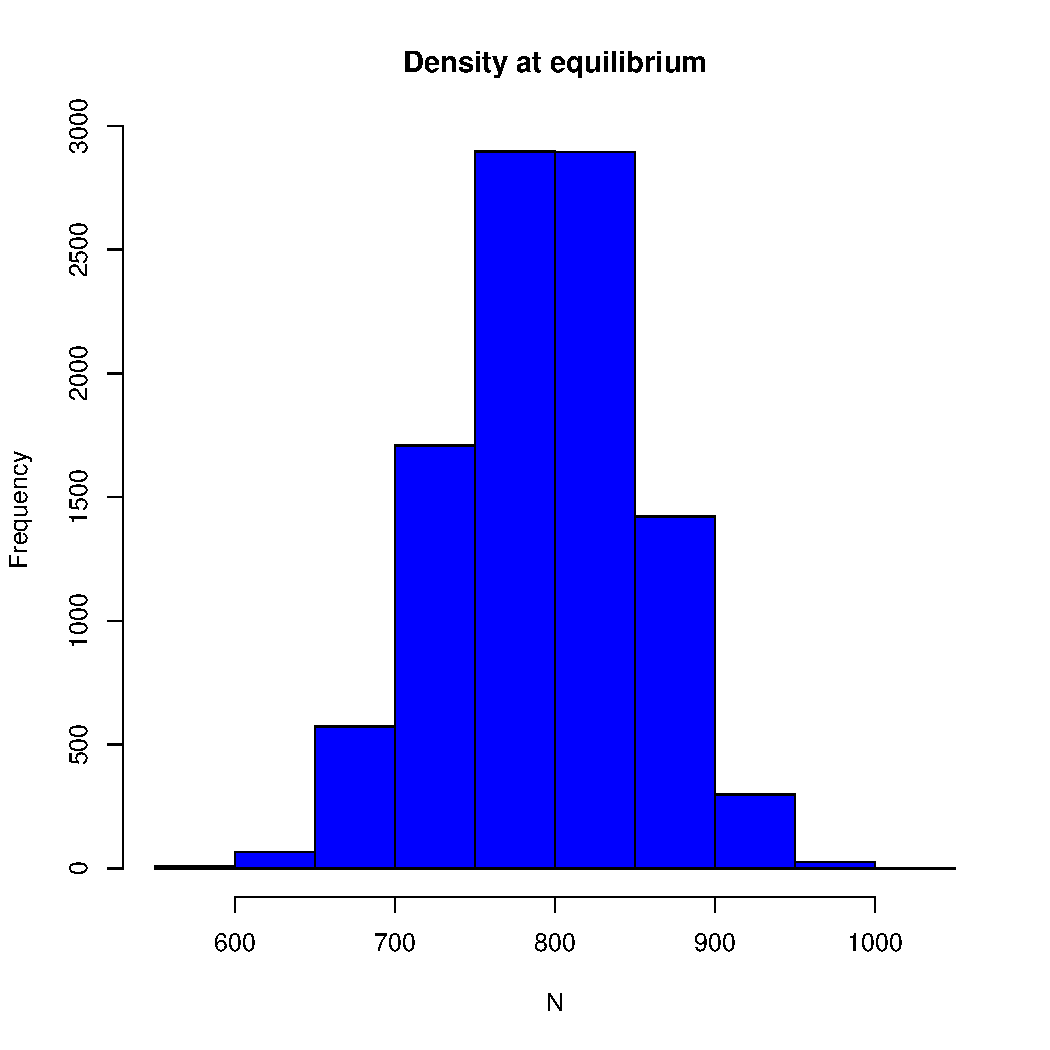
\includegraphics[width=0.3\linewidth]{../output/PreBSE/N_equil/Empirical_Dist_Neq} }}%
	\qquad
	\subfloat[\textbf{During} the BSE outbreak] {{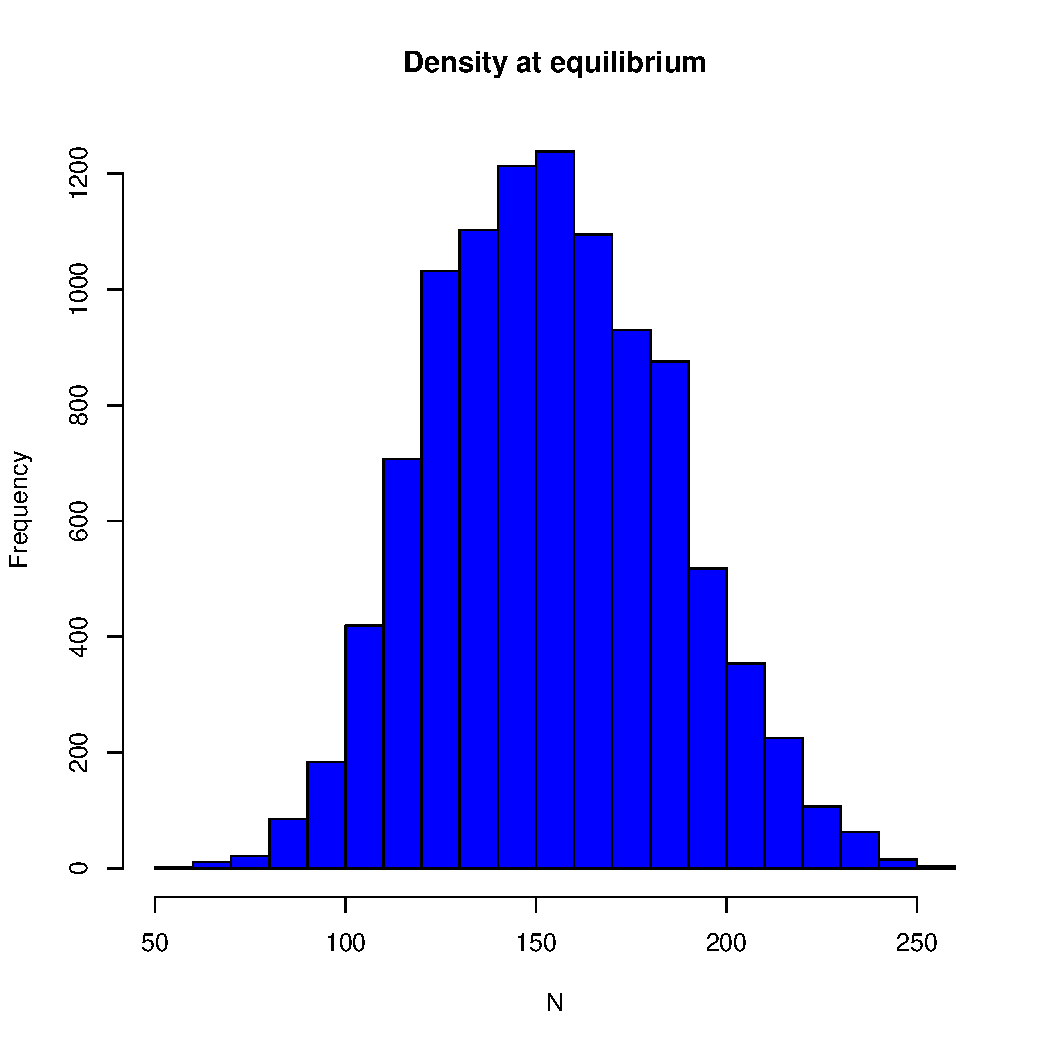
\includegraphics[width=0.3\linewidth]{../output/BSE/N_equil/Empirical_Dist_Neq} }}%
	\qquad
	\subfloat[\textbf{After} the BSE outbreak] {{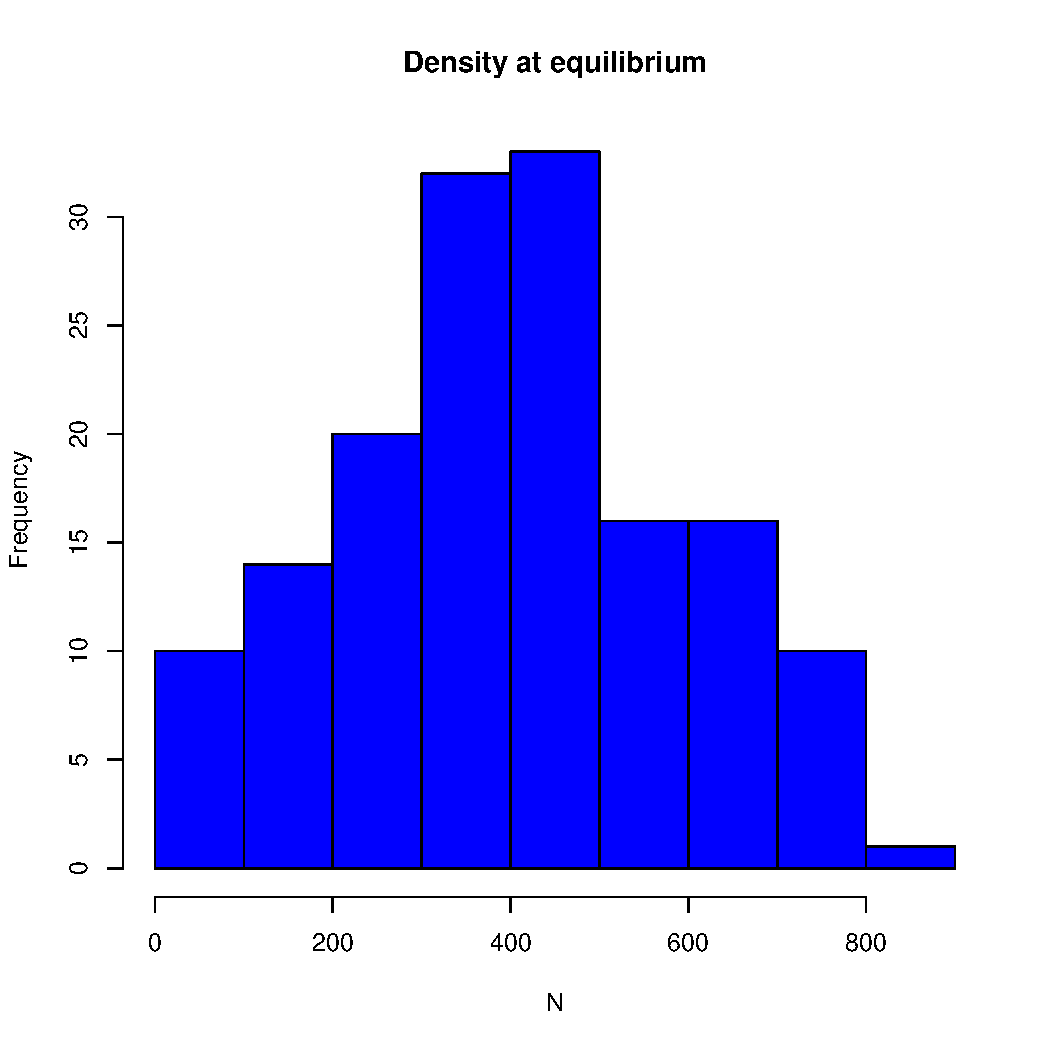
\includegraphics[width=0.3\linewidth]{../output/PostBSE/N_equil/Empirical_Dist_Neq} }}%
	
	\caption{Posterior distributions of the density at equilibrium ($N^*$) before (\textbf{a}), during (\textbf{b}) and after (\textbf{c}) the BSE outbreak.}%
	\label{fig:Neqs}%
\end{figure}

\renewcommand{\thefigure}{S3}
\begin{figure}[htbp]
	\begin{center}
		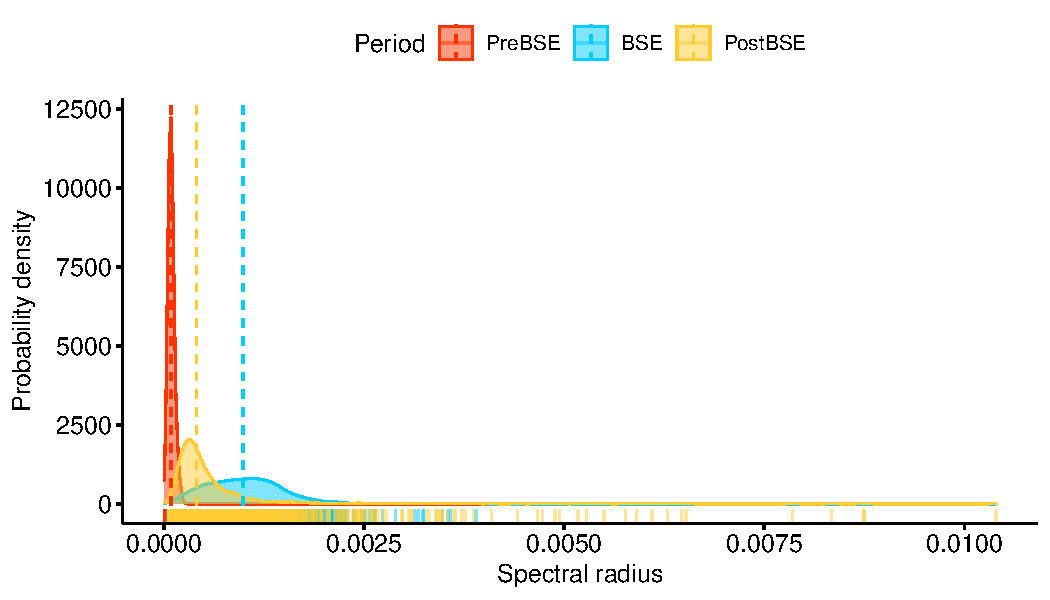
\includegraphics[width=10cm]{figs/FigS3.pdf}
	\end{center}
	\caption{Posterior distributions of the spectral radius, the modulus of the dominant eigenvalue of the Jacobian (eqn. \ref{Jacobian}) of the S4D3M evaluated at the equilibrium $N^*$, for the three time periods considered. PreBSE: before the BSE outbreak (1978-2001; BSE: during the BSE outbreak (2002-2011); and PostBSE, after the BSE outbreak (2012-2020)).}
	\label{fig:Asympt_resil}
\end{figure}

\section{Testing the performance of the model on simulated data}

The stage-structured demographic model we propose is structurally identifiable \cite{Bellman1970,Cole2020,Villaverde2016}: the Lefkovitch matrix is full-rank, and all of the parameters are conditioned on data. This means that, given sufficient data, all the demographic parameters, process variances and latent states can be recovered with accuracy. However, in real situations there might be issues with parameter identifiability due to, e.g., low sample sizes \cite{Cole2020}. In contrast to structural identifiability, this is called practical non-identifiability. To evaluate this potential problem, we build two synthetic scenarios in which a large number of stochastic time series are generated from models with known demographic parameters and stochastic effects. The S4D3M model is then fitted to each of these synthetic time series using the same Bayesian approach described in the accompanying paper. If the fitted parameter values correlate strongly with the ground-truth values, this would be strong evidence that the S4D3M is strongly identifiable in practice.\\

In the first scenario, we consider a process model with density-independent demographic dynamics with the following parameter values:

\begin{align}\label{FullModel_DI}
	\left(\begin{array}{c}
		{n_{f, t}} \\ 
		{n_{s, t}} \\ 
		{n_{a, t}}
	\end{array}\right)=
	\left(\begin{array}{ccc}{0} & {0} & {0.5} \\
		{0.25} & {0.4} & {0} \\
		{0} & {0.6} & {0.95}
	\end{array}\right)
	\times\left(\begin{array}{c}
		{n_{f, t-1}} \\ 
		{n_{s, t-1}} \\ 
		{n_{a, t-1}}
	\end{array}\right)+ \notag \\
	MVN\left(0,\left(\begin{array}{ccc}
		{62.5} & {-37.5} & {-12.5} \\
		{-37.5} & {62.5} & {-12.5} \\
		{-12.5} & {-12.5} & {62.5}
	\end{array}\right)+\left(\begin{array}{ccc}
		{\frac{25}{n_{f, t}}} & {0} & {0} \\
		{0} & {\frac{25}{n_{s, t}}} & {0} \\
		{0} & {0} & {\frac{25}{n_{a, t}}}\end{array}\right)\right)\end{align}

In the second scenario, we consider a process model with density-dependent fecundity:

\begin{align}\label{FullModel_DD}
	\left(\begin{array}{c}
		{n_{f, t}} \\ 
		{n_{s, t}} \\ 
		{n_{a, t}}
	\end{array}\right)=
	\left(\begin{array}{ccc}{0} & {0} & {\frac{0.5}{1+0.001N_{t-1}}} \\
		{0.25} & {0.4} & {0} \\
		{0} & {0.6} & {0.95}
	\end{array}\right)
	\times\left(\begin{array}{c}
		{n_{f, t-1}} \\ 
		{n_{s, t-1}} \\ 
		{n_{a, t-1}}
	\end{array}\right)+ \notag \\
	MVN\left(0,\left(\begin{array}{ccc}
		{62.5} & {-37.5} & {-12.5} \\
		{-37.5} & {62.5} & {-12.5} \\
		{-12.5} & {-12.5} & {62.5}
	\end{array}\right)+\left(\begin{array}{ccc}
		{\frac{25}{n_{f, t}}} & {0} & {0} \\
		{0} & {\frac{25}{n_{s, t}}} & {0} \\
		{0} & {0} & {\frac{25}{n_{a, t}}}\end{array}\right)\right)\end{align}

In both scenarios, the same observation equations were used:

\begin{equation}\label{ObsEqns2}
	\begin{array}
		{l}{y_{f, t} \sim \mathcal{P}(n_{f, t})} \\
		{y_{s, t} \sim \mathcal{P}(n_{s, t})} \\
		{y_{a, t} \sim \mathcal{P}(n_{a, t})}
	\end{array}
\end{equation}

The same initial values were used for all \textit{i} stages: 50 adults, 40 sub-adults and 100 fledglings.\\

We simulated an ensemble of 100 time series in each scenario during a 30 year period. The results of the Bayesian fittings of the S4D3M model to each synthetic time series is shown in Figure \ref{fig:FigSupp_PPC}. Even in the presence of relatively large amounts of process stochasticity and sampling variability, the distribution of the posterior estimates of the demographic rates obtained from the fitting of the S4D3M to the ensemble of synthetic time series correlate strongly with their ground-truth estimates, in both the density-independent and density-dependent fecundity scenarios. These results suggest that the S4D3M is strongly identifiable in practice.\\


\renewcommand{\thefigure}{S4}
\begin{figure}[htbp]
	\begin{center}
		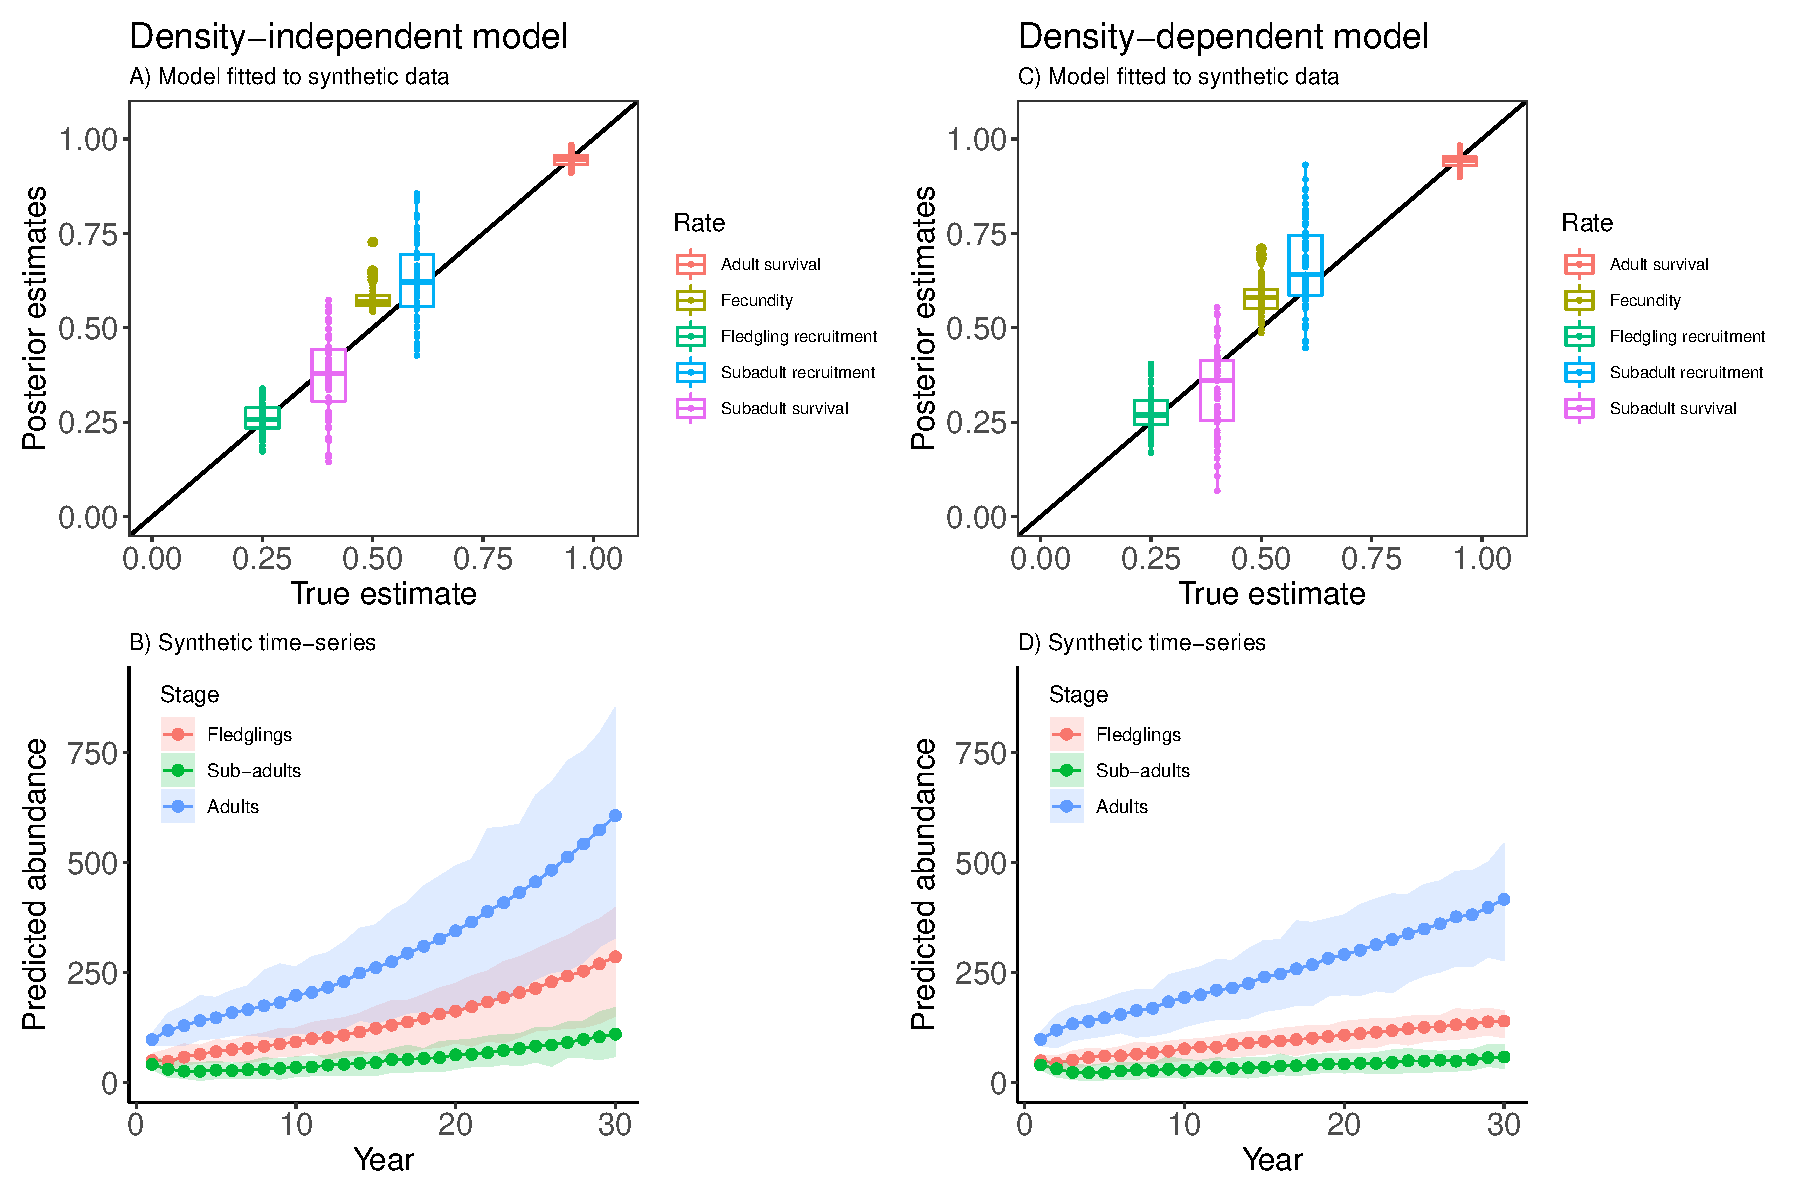
\includegraphics[width=15cm]{figs/FigS4.pdf}
	\end{center}
	\caption{Results of the stochastic simulation testing the practical identifiability of the S4D3M model from synthetic scenarios. A) and B) show the results of the density-independent scenario (model \ref{FullModel_DI}), while C) and D) show the results for the density-dependent fecundity scenario (model \ref{FullModel_DD}). In A) and C) the posterior estimates for the vital rates of the S4D3M fitted to each of the 50 synthetic time-series are plotted against the ground-truth values for the density-independent and density-dependent synthetic scenarios, respectively. The box-plots show the median (horizontal line), inter-quantile range (box) and 95\% percentiles (whiskers). The thickness of the box is proportional to the posterior density of the estimates within the inter-quantile range. The Y=X regression line (in black) is plotted as a reference. Sub-figures B) and D) show the average of the 100 time series of abundances for the three demographic stages simulated from the density-independent and density-dependent fecundity synthetic scenarios, respectively. The average of the synthetic time series are shown for each stage as lines and shaded regions stand for the 95\% confidence interval. }
\label{fig:FigSupp_PPC}
\end{figure}

\newpage

\pagestyle{empty}
\begin{landscape}

\section{Supplementary Tables}

	\begin{table}[!htbp]
		\centering
		\caption{Summary of vital rates estimates for the Eurassian Gryfon vulture (\textit{Gyps fulvus}) obtained in several areas of the western Paleartic.}
		\label{t_sim}
		\begin{tabular}{cccccccc}
			\toprule
			\thead{Fecundity} & \thead{\makecell{Fledgling \\ recruitment}} & \thead{\makecell{Sub-adult \\ recruitment}} & \thead{\makecell{Sub-adult \\ survival}} & \thead{\makecell{Adult \\ survival}} & \thead{Location} & \thead{Comment} & \thead{Reference} \\
			\midrule
			0.818 & 0.6462 & - & 0.9485 & \makecell{0.9463 \\ 0.9485 \\ 0.8240 ($>$ 28 years)} & \makecell{Grand Causses, \\ Massif Central, \\ France} & \makecell{Late onset of senescence ($>$ 28 years).\\ Different adult annual survivals \\ depending on assumed model.}  & \cite{Chantepie2016a} \\
			\hline
			- & - & - & 0.858 & 0.987 & \makecell{Grand Causses, \\ Massif Central, \\ France} & \makecell{A release effect on adult survival \\ was detected (0.743 during first year).} & \cite{Sarrazin1996} \\
			\hline
			0.785 & 0.871 & - & - & - & \makecell{Grand Causses, \\ Massif Central, \\ France} & \makecell{Average figures for of 11 years. \\ Only for first clutches.} & \cite{Sarrazin2000} \\
			\hline
			0.740 & - & - & - & - & \makecell{Island of Crete, \\ Greece} & \makecell{5 years of monitoring.} & \cite{Xirouchakis2010} \\
			\hline
			0.698 & - & - & - & - & \makecell{25 areas of the \\ western Paleartic.} & \makecell{Figure is the average for \\ 25 areas of the western Paleartic. \\ Range: 0.450-0.890} & \cite{Xirouchakis2010} \\
			\hline
			0.770 & 0.710 & - & - & - & \makecell{Eastern Rhodopes, \\ Bulgaria} & \makecell{25-year survey of two sites.} & \cite{Demerdzhiev2014} \\
			\hline
			- & - & - & 0.955-0.970 & 0.955-0.970 & \makecell{Causses, Baronnies, \\ Verdon, Navacelles, \\France} & \makecell{Range of long-term survival rates \\ with release-recapture models.} & \cite{Gouar2008a} \\
			\hline
			0.670-0.710 & 0.560-0.60 & - & - & - & \makecell{Esla, Porma, \\ Picos de Europa, \\ Spain} & \makecell{41 pairs monitored \\ during year 1997.} & \cite{OleaGarciaFalagan1999} \\
			\hline
			- & 0.688 & - & 0.946-0.964 & 0.952-0.969 & \makecell{Several areas, \\ Northeast Portugal} & Data from sensitivity analysis & \cite{VanBeest2008} \\
			\bottomrule
		\end{tabular}
	\end{table}
\end{landscape}
\newpage

	\begin{table}[!htbp]
		\centering
		\caption{\label{t_dd} Probability of density-dependence in vital rates and associated Bayes factors for each time period. Note that the prior probability of inclusion of the density-dependent parameter in the stage-structured demographic model is common to all vital rates for each time period. In bold type, vital rates for which the Bayes factor suggest that evidence of density-dependence for that rate is barely worth mentioning (1 to 3.2) according to the Kass-Raftery scale \cite{Kass1995}. }
		\begin{tabular}{cccccccccc}
		\toprule
			\multirow{1}{*}{\textbf{Vital rate}} &
			\multicolumn{3}{c}{\textbf{Pre-BSE}} &
			\multicolumn{3}{c}{\textbf{BSE}} &
			\multicolumn{3}{c}{\textbf{Post-BSE}} \\
			& \textbf{Prior} & \textbf{Posterior} & \textbf{Bayes factor} 
			& \textbf{Prior} & \textbf{Posterior} & \textbf{Bayes factor} 
			& \textbf{Prior} & \textbf{Posterior} & \textbf{Bayes factor} \\
			\hline
			\thead{Fecundity}  & 0.280 & 0.016 & 0.043 & 0.264 & 0.012 & 0.034 & 0.255 & 0.014 & 0.042 \\
			\hline
			\thead{\makecell{Fledgling \\ recruitment}} & 0.280 & 0.014 & 0.037 & 0.264 & 0.018 & 0.052 & 0.255 & 0.015 & 0.044 \\
			\hline
			\thead{\makecell{Sub-adult \\ survival}} & 0.280 & \textbf{0.466} & \textbf{2.248} & 0.264 & 0.064 & 0.191 & 0.255 & 0.023 & 0.068 \\
			\hline
			\thead{\makecell{Sub-adult \\ recruitment}} & 0.280 & 0.019 & 0.049 & 0.264 & 0.241 & 0.882 & 0.255 & 0.207 & 0.766 \\
			\hline
			\thead{\makecell{Adult \\ survival}} & 0.280 & 0.018 & 0.046 & 0.264 & 0.014 & 0.039 & 0.255 & 0.015 & 0.045 \\
			\bottomrule
		\end{tabular}
	\end{table}

\newpage

\printbibliography

\end{document}
